\section{Fragen}
\subsection*{Woche 2}
\textbf{Hauptaufgabe der Control Unit (CU)?} \newline
It tells the computer's memory, arithmetic/logic unit and input and output devices how to respond to a program's instructions.\newline


\textbf{Hauptaufgabe der Central Processing Unit (CPU)?} \newline
    Fetches, decodes, and executes instructions from memory\\
 
\textbf{Was ist die Verarbeitungsbreite?}\newline
    Breite welcher in der Alu mit einem Takt verarbeitet werden kann, meistens gleich der Register- und der Datenbusbreite.\\
    
\textbf{What is a Power on Reset (POR)?}\newline
    A signal to bring the CPU and peripherals to an initial, known state designated as the RESET state\newline
    A requirement for all sequential circuits\newline
    Generated by a dedicated POR circuit\\

\textbf{Effects of a Valid POR on a CPU?}
\begin{enumerate}
    \item Loads the Program Counter (PC) with the address of the first  instruction to be fetched (boot sequence)
    \item Disables the reception of Maskable Interrupts
    \item Clears the Status Register (SR)
    \item Resets some or all system peripherals
    \item Cancels any bus transaction in progress and returns control to the default bus master.
\end{enumerate}

\subsection*{Woche 3}
Adressbusbreite n: ergibt maximal ansprechbare Speicherstellen ($2^n$)\newline
    
\textbf{Wieviele Adressen sind ansprechbar? MSP430 / MSP430X}\newline
    MSP 430  \qquad 16bit $ \rightarrow $ 64kbit \newline
    MSP 430X \quad 20bit $ \rightarrow $ 1mbit \newline
    
    Von Neumann und little Endian
    
\subsection*{Woche 4}
\textbf{Was macht ein Adressdecoder?}\newline
    nimmt das MSB der Adressleitung um zwischen den Speicherchips zu wechseln.\\
    
\textbf{Welchen nutzen hat der linearregler nach dem DC/DC Wandler?}\newline
    Reduziert die Brummspannung des DC/DC Wandlers.
    
\subsection*{Woche 5}
\textbf{Erläutern sie das Konzept der Adressdekodierung.}\newline
    
\textbf{Speichergrösse bei Adressbereich von 0x09000 bis 0x0B3FF?}\newline
\[ 0h0B3FF - 0h09000 = 0h023FF \rightarrow 9215Byte \]
\textbf{Speichergrösse bei Adressbereich von 0x0400 bis 0x17FF?}\newline
\[ 0h17FF - 0h0400 = 0h13FF \rightarrow 5119Byte \]
\textbf{Peripherieeinheiten verfügen in der Regel über  3 verschieden Register?}\newline
\begin{tabular}{ll}
    Control & to configure the operation of the device \& interface\\
    Status  & to allow inquires about the device \& interface status\\
    Data    & for exchangeing data woth the device
\end{tabular}

\subsection*{Woche 7}
\textbf{Unterschiede \& Gemeinsamkeiten zwischen Exception und Interrupt?}\newline
    \null\qquad \textbf{Interrupt}
    \begin{itemize}
        \item A Signal wich indicates an event whiche needs immidiate CPU attention
        \item Can occure in Peripherie
    \end{itemize}
    
    \qquad \textbf{Exceptions}
    \begin{itemize}
        \item Generated by the CPU
        \subitem CPU State, Division by Zero, Overflow
        \item non maskable
    \end{itemize}

\textbf{Welche Info steht an der Adresse 0x0FFFC des MSP430?}\newline
    Reset- Vektor
    
\textbf{Was versteht man unter dem Begriff Auto-Vectored-Interrupt?}\newline
    ISRs welche nicht in eine Jumplist (Vektortabelle) eingetragen werden muss.\\

\textbf{Wie wird der Low-Power-Mode beim MSP430 aktiviert?}\newline
    Setzen der Flags im Statusregister.\\
    
\textbf{Wodurch kann die CPU aus dem LPM in den AktivMode gebracht werden? temporär, dauerhaft?}\newline
    temporär durch Interrupt \newline
    dauerhaft durch löschen der Flags in einer ISR oder nach dem POR\\
    
\textbf{Begriffe Erklären der seriellen Kommunikation?}\newline
\null\qquad \textbf{Simplex}\newline
    Unidirectional Link,Only one direction, no ACK of Data\newline
    
\qquad \textbf{Half Duplex}\newline
    One bidirectional Link, both directions, one direction at one Time\newline
    
\qquad \textbf{Full Duplex}\newline
    Two seoeratet bidirectional Links, both directions, Simultanouse Communication\newline
    
\qquad \textbf{Single Ended}\newline
    Asymetrische Datenübertragung.\newline
    One wire carries a varying voltage, the other wire a reference voltage.\newline
    
\qquad \textbf{Differential}\newline
    Receiving circuit responds to the electrical difference between two signals.
\clearpage
\subsection*{Woche 8}
\textbf{Was versteht man unter einem Null-Modem?}\newline
     RX,TX gekreuzt um 2 Endgeräte zu verbinden. Hand-Shake Leitung\\
     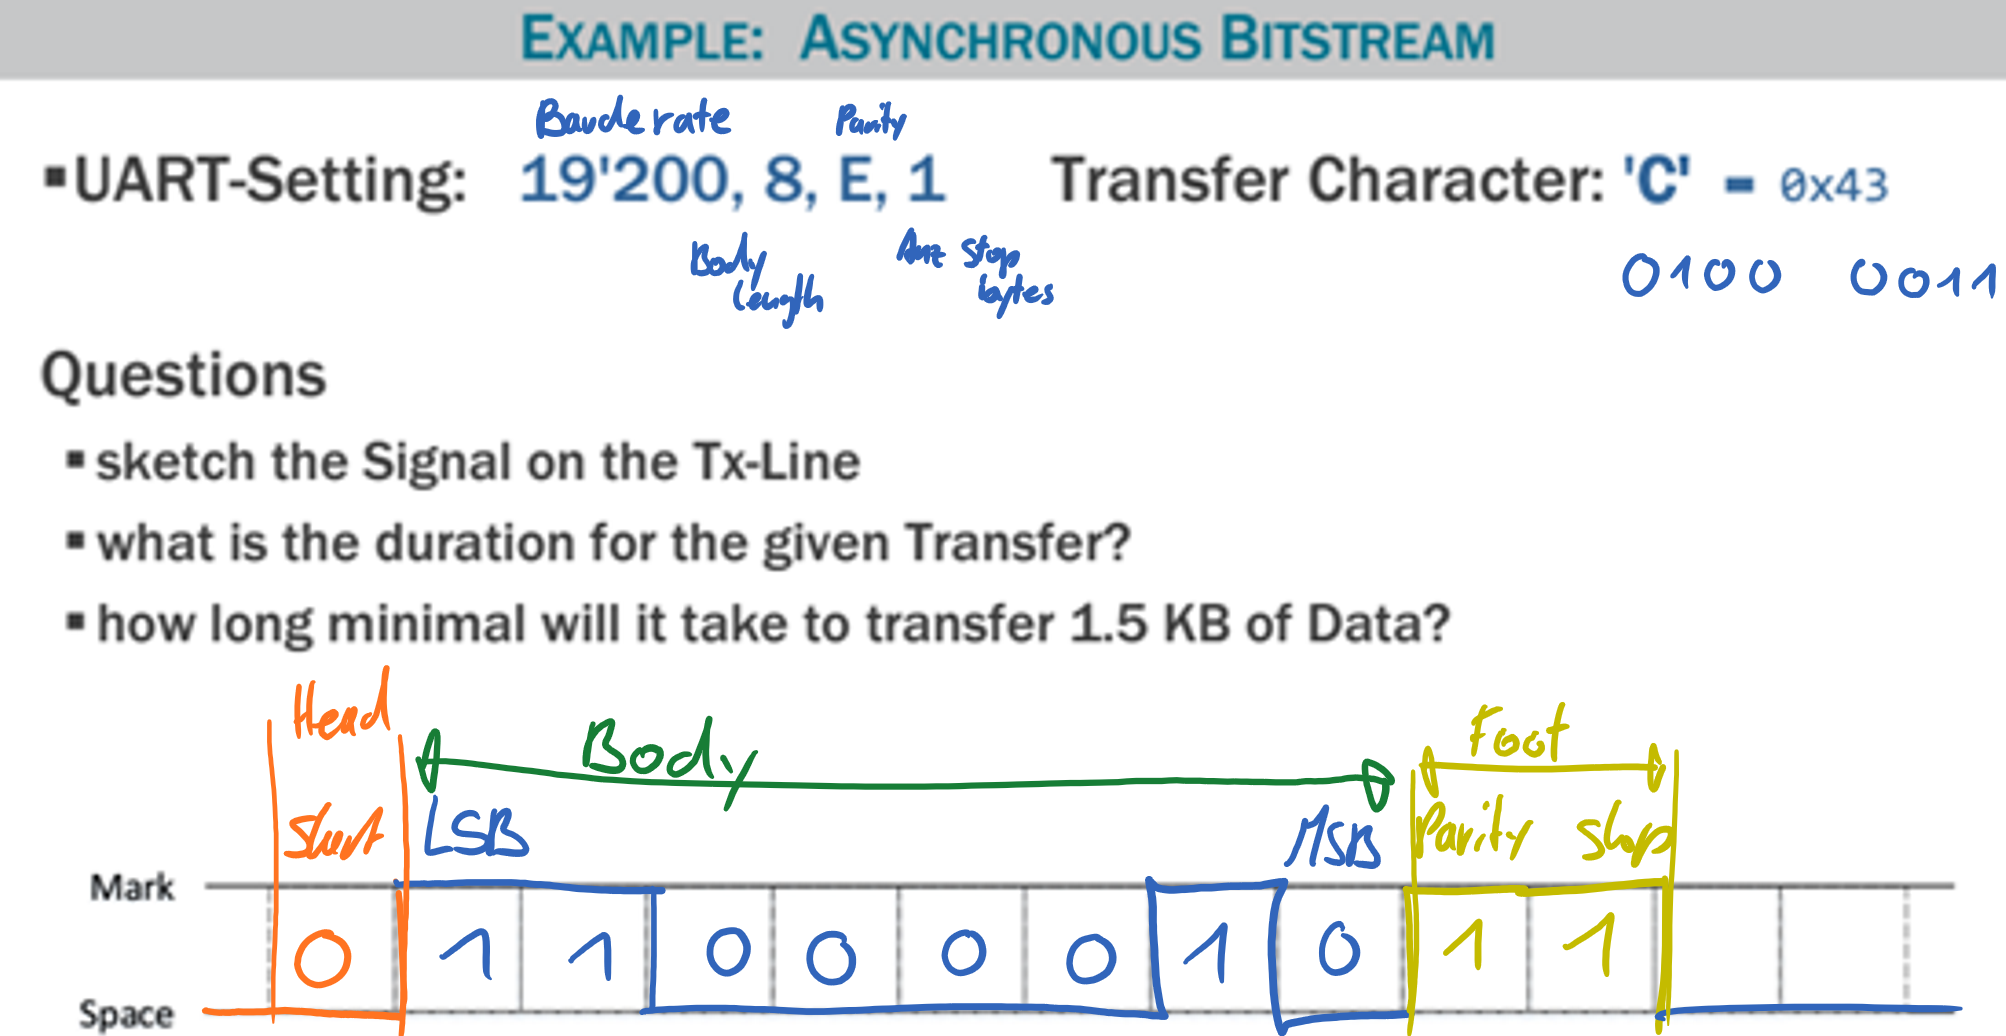
\includegraphics[width=10cm]{images/FragenUart}\newline
     
     \textbf{duration}\newline   
     
\subsection*{Woche 9}
\textbf{Eräutern sie die Funktion und die Notwendigkeit von Ringbuffern?}\newline
    Für Datenübertragung zwischen zwei Asynchronen Teilnehmern\newline

\textbf{UART vs. RS232}\newline
\null\qquad \textbf{UART}\newline
    UART nicht definierte Logik-Pegel\newline
\null\qquad \textbf{RS232}\newline
    RS-232 ist UART-Schnittstelle mit definiertem Pegel
    
\subsection*{Woche 10}
\textbf{Erläutern sie das XON / XOFF Handshake Verfahren}\newline
    Möglichkeit zu garantieren dass der Buffer nicht überläuft\newline
    Andere Möglichkeit wäre CTS (Handshakeleitungen)\newline
    
\textbf{Welche Signalleitungen sind für eine unidirektionale Bus Verbindung von einem SPI Master zu einem SPI Slave minimal erforderlich?}\newline
    SCLK, MOSI, GND

\subsection*{Woche 11}
\textbf{Wie kann ein Busteilnehmer auf dem $I^2C$-Bus die Geschwindigkeit der Datenübertragung reduzieren?}\newline
    Jeder Teilnehmer hat die möglichkeit die SCLK Leitung zu manipulieren, wait-states einzufügen(auf GND halten)
    
\subsection*{Woche 12}
\textbf{Aufgrund welcher Information erfolgt beim $I^2C$ die Bus-Arbitrierung (Buszuteilung)?}\newline
    Tiefste Adresse bei gleichzeitigem Zugriff\newline
    
\textbf{Wie erfolgt beim SPI-Bus die Bus-Arbitrierung?}\newline
    Slave select\newline
    
\textbf{Wie erfolgt bei einer UART die Bus-Arbitrierung?}\newline
    nur zwei teilnehmer\newline
    
\textbf{Wie erfolgt beim RS-485 die Bus-Arbitrierung?}\newline   
    haben nur einen Master
    
\subsection*{Woche 13}    
\begin{itemize}
    \item wie funktioniert ein SAR ADC?
    \item wie funktioniert ein single-Slope ADC?
    \item wie funktioniert ein dual-Slope ADC?
\end{itemize}

\section*{Mögliche Prüfungsinhalte}
Aufgaben vor allem zu Themen aus Praktikas:
\begin{itemize}
\item Schnittstellen kennen: SPI, UART, I2C
\subitem Dauer der Übertragung, Signalform Bitmuster übertragen mit gegebener Parität/Datenrate etc.

\item Batterielebensdauer berechnen

\item Speichersysteme
\subitem Dekodieren von Adressbereichen, Little Endian/Big Endian :D

\item Watchdog
\subitem Theoretische Fragen: Wieso gibt es diesen? Aufgabe? Schutzmechanismen MSP430…

\item Clocksystem

\item LowPower Mode:
\subitem Keine Frage wieviel uA braucht er sondern mehr wie das Umschalten funktioniert

\item PWM:
\subitem Berechnungen Zählstand/ Periodendauer etc mit vorgegebenem Clock

\item C-Code nur bedingt abgefragt
\subitem Interpretation, Lückentext (wie gehabt)

\item Timer:
\subitem Keine Frage zu Anzahl Timer des MSP430, Aber was wird benötigt um ihn richtig anzusteuern (z.B Sourceclock vorhanden, …)

\item Ringbuffer

\item ADC:
\subitem Wie funktioniert der ADC (Single Slope, Dual Slope)

\item Aufgaben zu Auflösung

\item DMA / Interrupt

\item I/O Pins eventuell Signalkonvertierungen kennen (Keine Schaltungsvorschläge erwartet)
\end{itemize}
Keine Musterlösungen für Kapitel 6/7/8/9/10 vorhanden, Aufgabenstellungen aus Buch gut zu überlegen aber diese kommen nicht 1:1 an der Prüfung (Fragen sind zu komplex, Buch wird benötigt um diese zu lösen -> Keine Zeit während der Prüfung)


















